\ProvidesFile{lecture01.tex}[Lecture 1]


\newpage

\section{Sets}

In modern math everything can be formulated in terms of Set Theory, that is in terms of sets and maps.
Let me remind some basic facts about sets and maps.

\subsection{Definition}

\begin{definition}
A set is a collection of elements.
\end{definition}

We denote sets by capital letters like $X$ and $Y$.
If an element $x$ belongs to the collection $X$, we write $x\in X$.
If $y$ does not belong to $X$, we write $y\notin X$.
There is a special set containing no elements.
This set is called an empty set and is denoted by $\varnothing$.

If you think of a set you should imagine a sack full of elements.
The sack is your set and the elements in the sack are the elements belonging to the set.
An empty set becomes a sack with no elements inside.

\subsection{Constructors}

If you are given a definition of a new math object, the first question to ask is: ``How do I construct such an object?'' To define a set we need to specify the elements inside the set.
For doing that, we use the following notation
\[
X = \{x\mid \text{\textbf{condition} on }x\}
\]
Here, we mean that the set $X$ consists of all elements $x$ such that the \textbf{condition} on $x$ holds.
Let me demonstrate this on examples.
\begin{itemize}
\item The set of natural numbers
\[
\mathbb N = \{x\mid x \text{ is a natural number}\} = \{0, 1, 2, 3, \ldots, n,\ldots\}
\]

\item The set of integer numbers
\[
\mathbb Z = \{x\mid x \text{ is an integer number}\} = \{\ldots,-2,-1,0,1,2,\ldots\}
\]

\item The set of real numbers
\[
\mathbb R = \{x\mid x \text{ is a real number}\}
\]
We think of the real numbers as a line containing all possible numbers we use in our calculations.

\item The closed interval $[0, 1]$
\[
[0, 1] = \{x\in \mathbb R \mid 0\leqslant x \leqslant 1\}
\]
Here, I use a slightly different notation.
I specified that $x\in \mathbb R$ before $|$, this simply means that $x$ must be a real number and the additional condition (the number is between zero and one) is written after $|$.

\end{itemize}


\subsection{Operations on sets}

There are several useful procedures you can apply to sets in order to construct new sets.
Let us discuss them.

\subsubsection{Intersection}

If we are given two sets $X$ and $Y$, then we define the intersection of $X$ and $Y$ as follows
\[
X \cap Y = \{z\mid z\in X\text{ and } z\in Y\}
\]
If we denote the sets $X$ and $Y$ by discs on a plain then the intersection of $X$ and $Y$ is denoted as below
\begin{center}
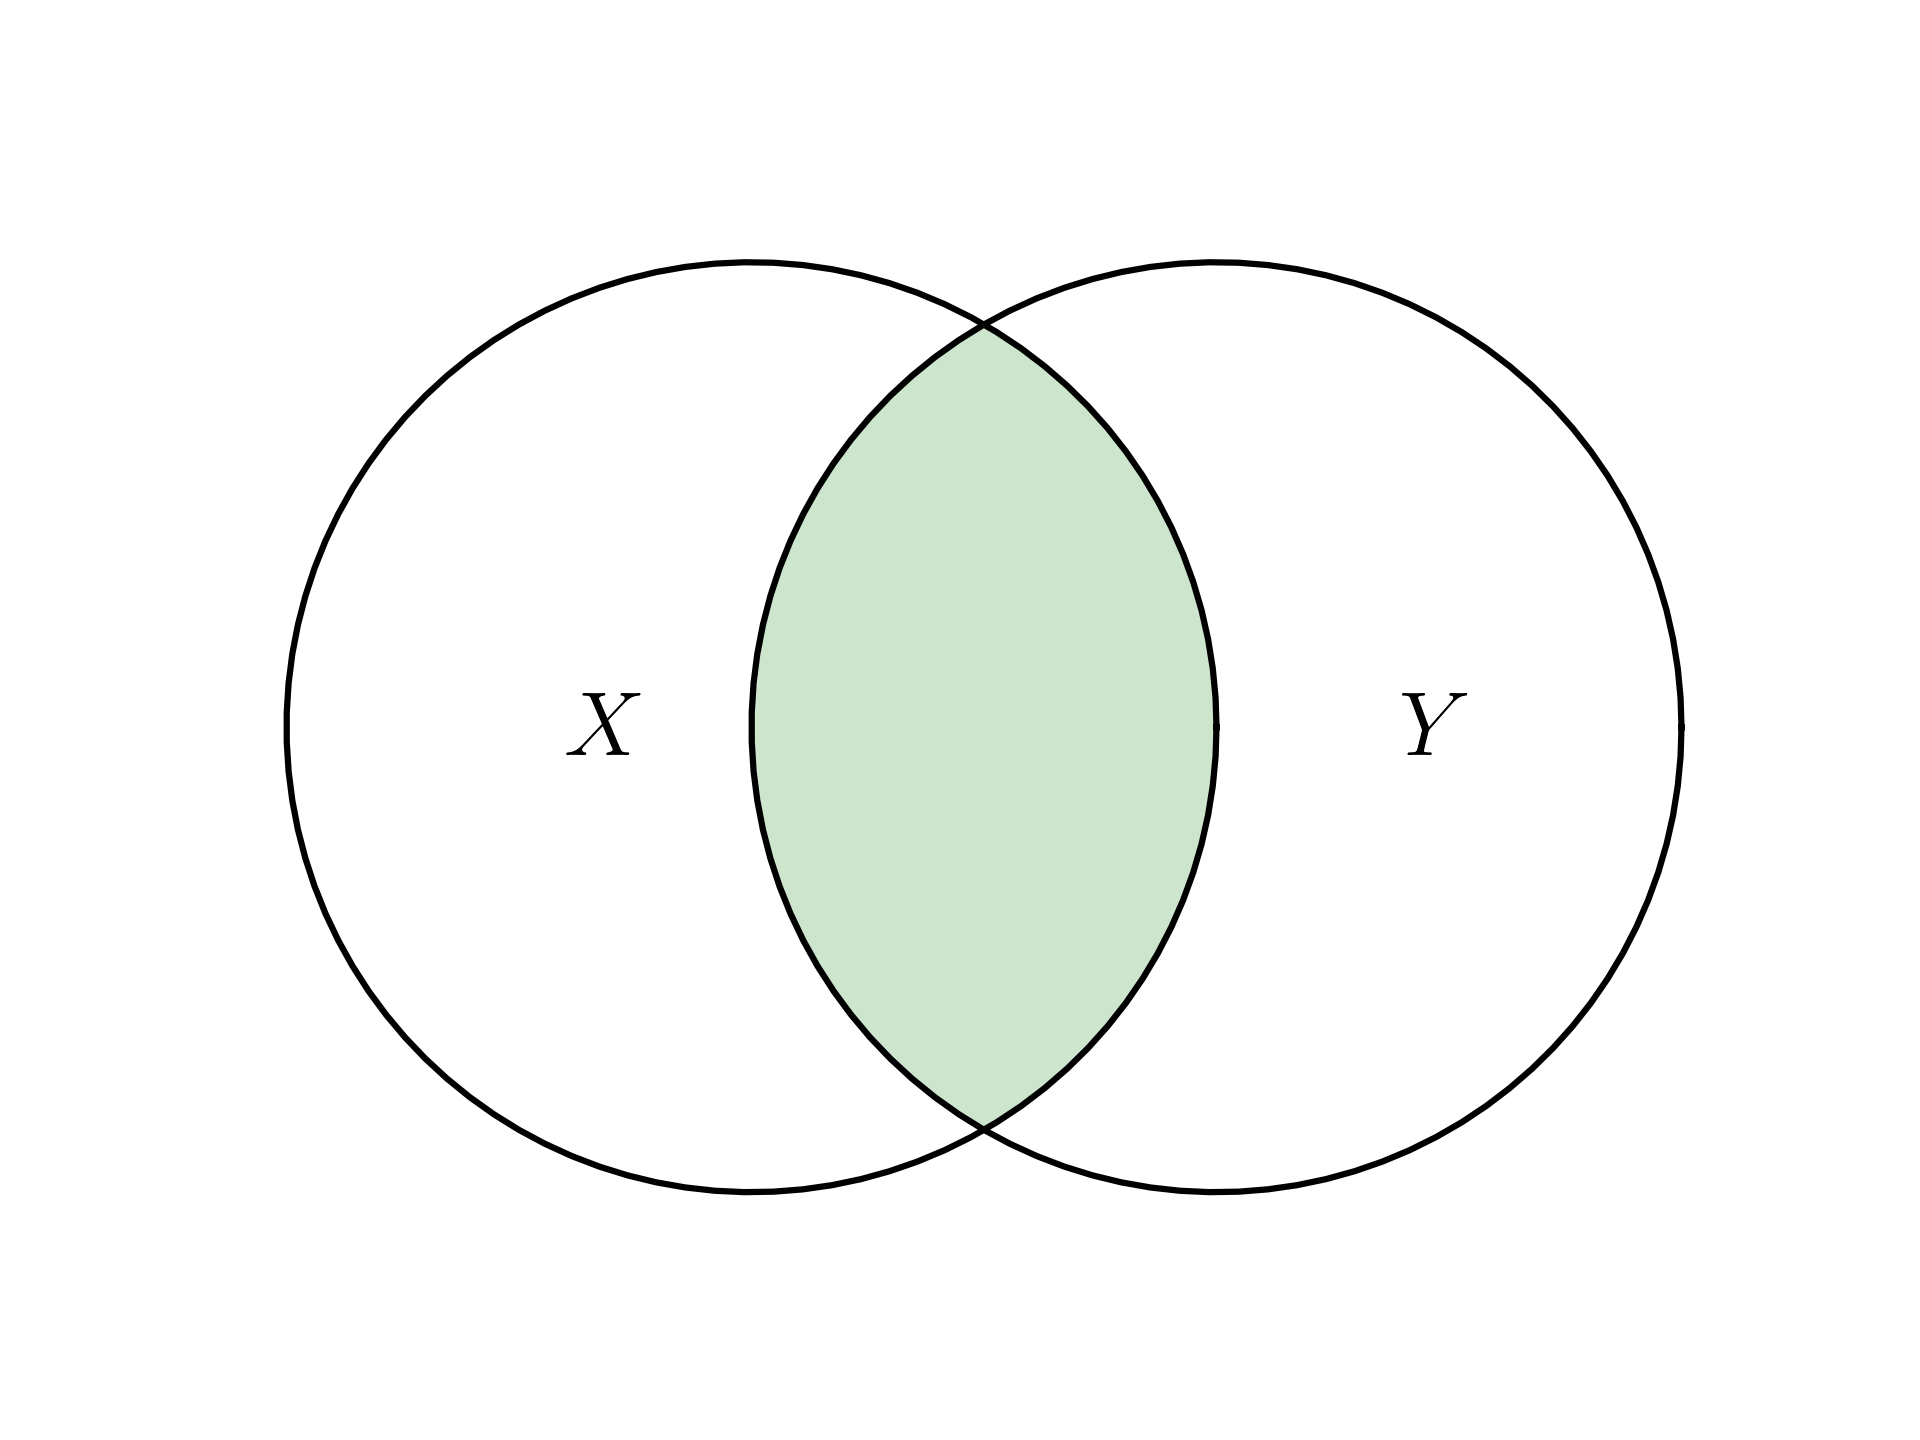
\includegraphics[scale = 0.3]{Figures/graph_intersection.png}
\end{center}

\subsubsection{Union}

If we are given two sets $X$ and $Y$, then we define the union of $X$ and $Y$ as follows
\[
X \cup Y = \{z\mid z\in X\text{ or }z\in Y\}
\]
If we denote the sets $X$ and $Y$ by discs on a plain then the union of $X$ and $Y$ is denoted as below
\begin{center}
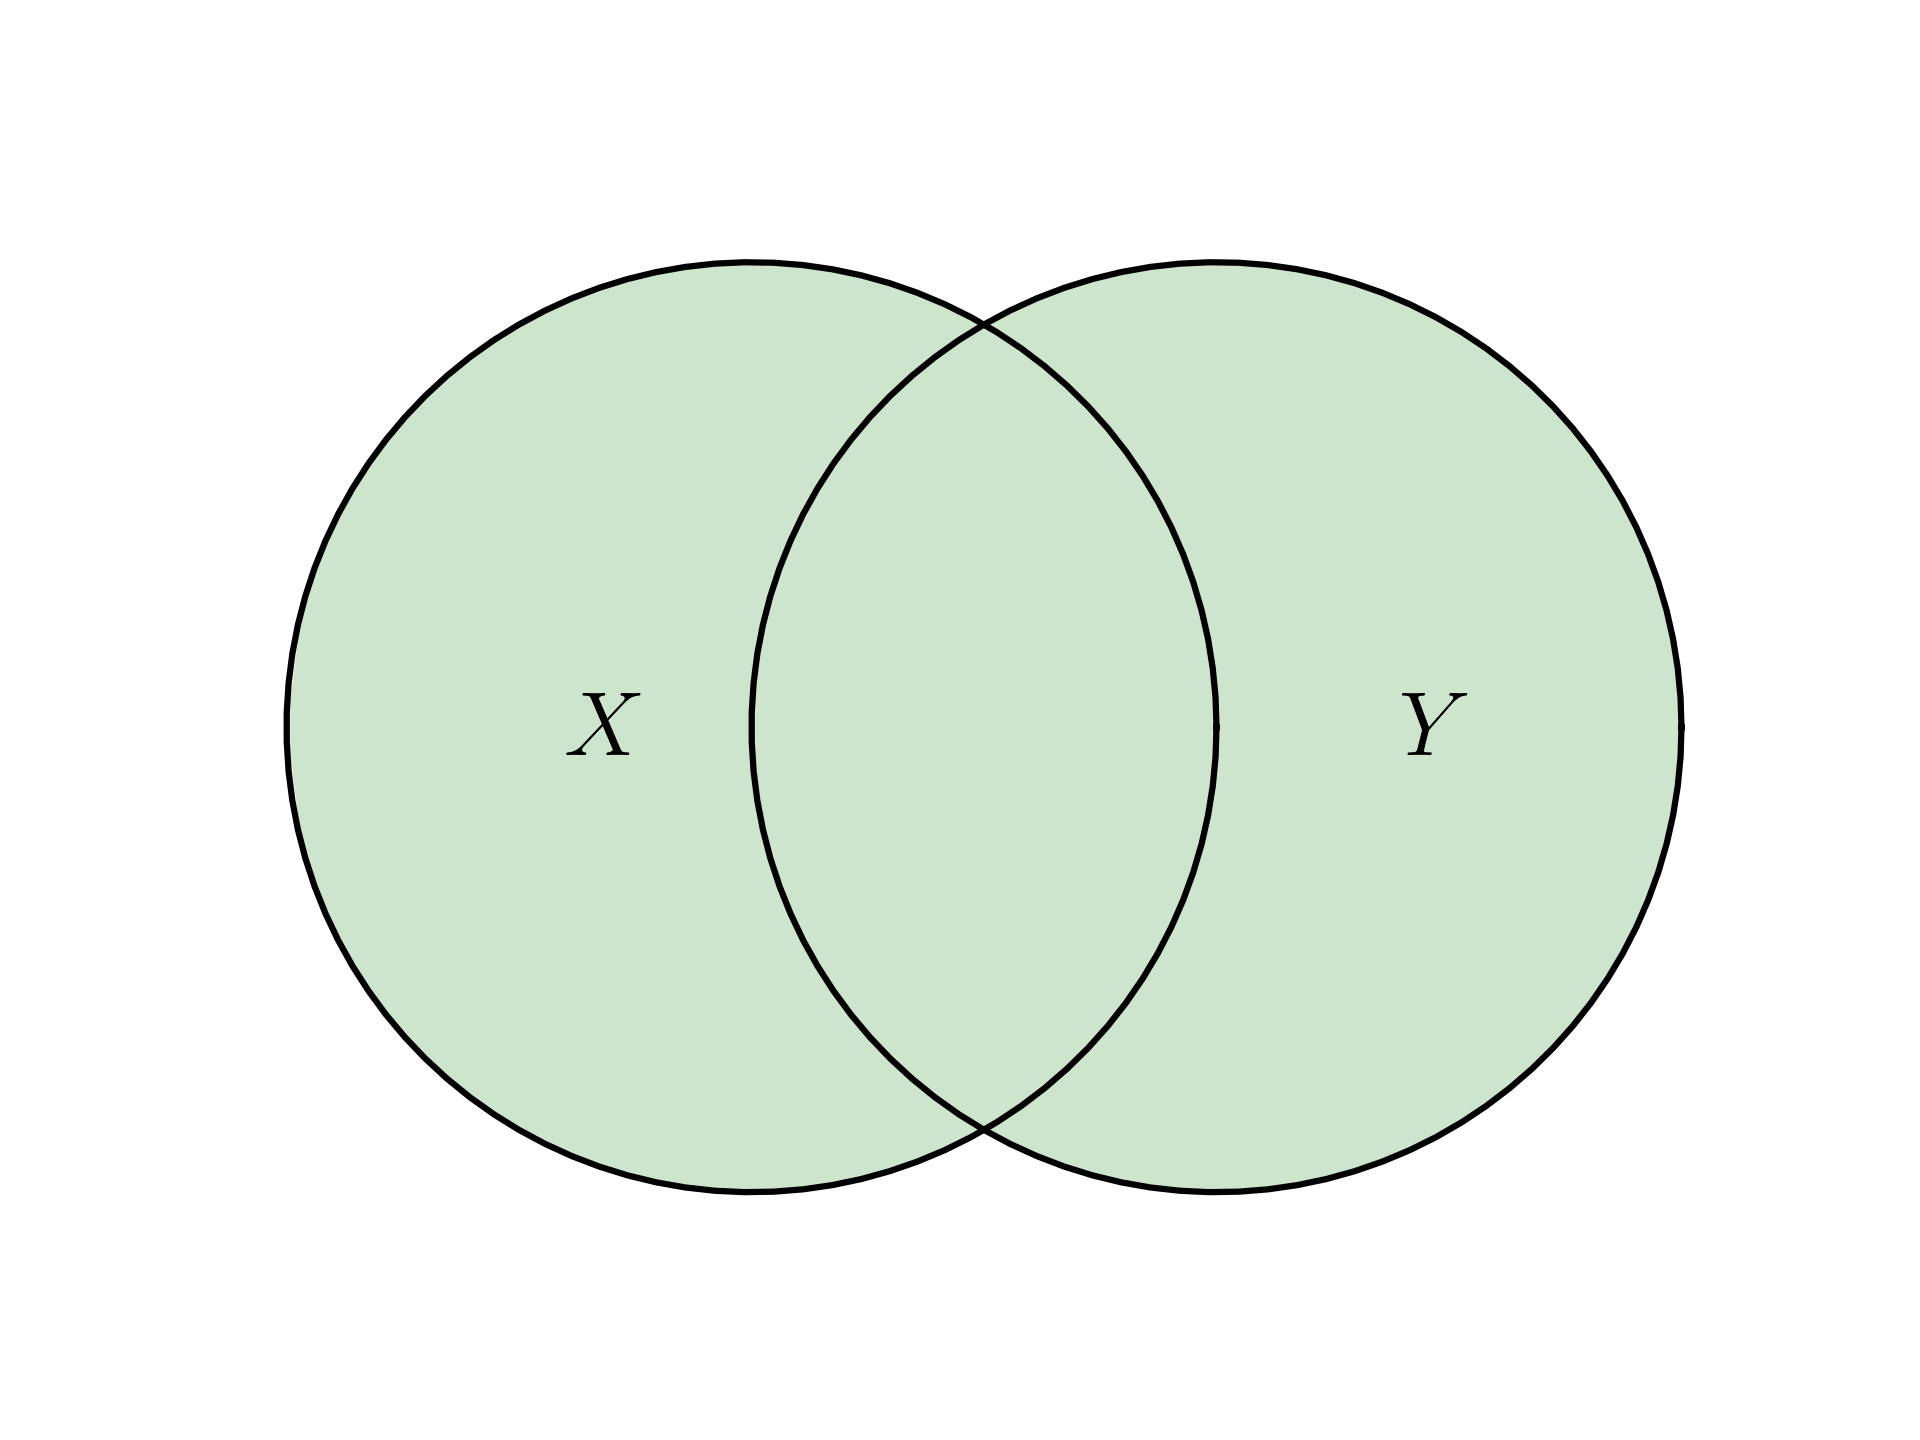
\includegraphics[scale = 0.3]{Figures/graph_union.png}
\end{center}

\subsubsection{Difference}

If we are given two sets $X$ and $Y$, then we define the difference between $X$ and $Y$ as follows
\[
X\setminus Y = \{z\mid z\in X\text{ and }z\notin Y\}
\]
If we denote the sets $X$ and $Y$ by discs on a plain then the difference between $X$ and $Y$ is denoted as below
\begin{center}
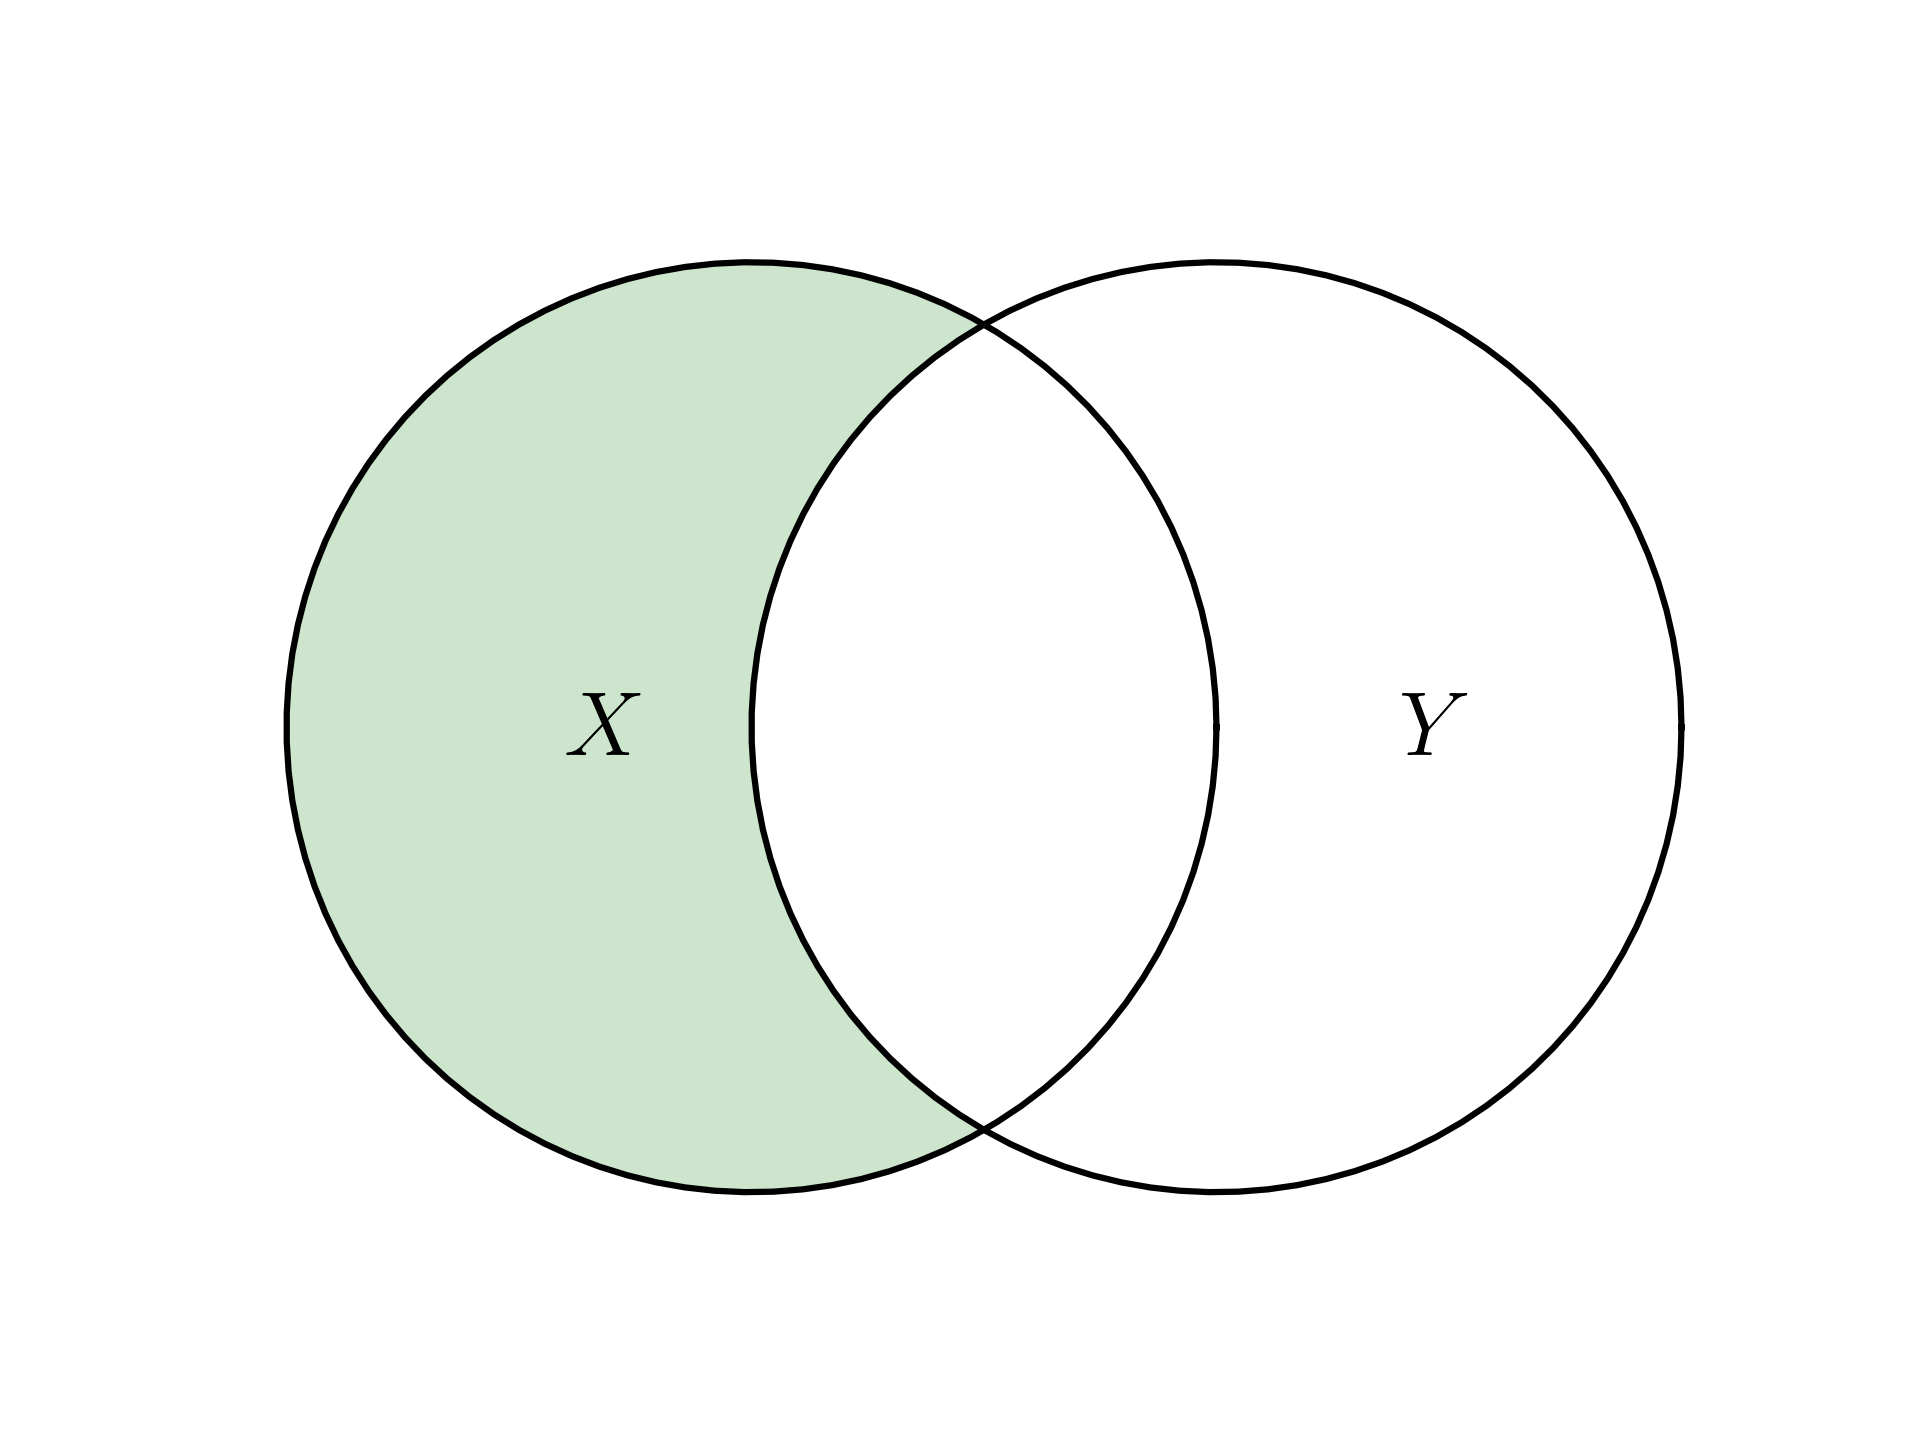
\includegraphics[scale = 0.3]{Figures/graph_difference.png}
\end{center}

\subsubsection{Cartesian product}

If we are given two sets $X$ and $Y$, then their Cartesian product is defined as follows
\[
X \times Y = \{(x, y)\mid x\in X,\;y\in Y\}
\]
The Cartesian product is simply the set of all possible pairs $(x, y)$ where the first element is taken from $X$ and the second from $Y$.
We will use it every time when we need pairs of elements and not just elements.
% TO DO
% Picture

\subsection{Maps}

\begin{definition}
Suppose we are given two sets $X$ and $Y$, a map $f\colon X\to Y$ is a rule that takes elements of $X$ to elements of $Y$.
If $x\in X$, then its image in $Y$ is denoted by $f(x)$.
In this case, we will write $x\mapsto f(x)$.
\end{definition}

The set $X$ is called the source of $f$ and the set $Y$ is called the target of $f$.

Here is a way to think about maps.
Suppose we are given a map $f\colon X\to Y$.
Then $f$ is a callable object with an operator $({-})$.
You give it any element $x$ of $X$, then it returns you some specific element $f(x)$ of $Y$.
For each input $x\in X$, the result $f(x)\in Y$ will be the same every time you call it.
So, a map is the same thing as a function.

\begin{examples}
Here are some examples of maps and non maps.
\begin{enumerate}
\item The rule $f\colon \mathbb R\to \mathbb R$ by $x\mapsto 2 x + 3$ is a map.

\item The rule $f\colon \mathbb R\to \mathbb R$ by $x\mapsto \sin(x)$ is a map.

\item The rule $f\colon \mathbb R\to \mathbb R$ by $x\mapsto \frac{1}{x}$ is not a map because it is not defined at $x = 0$.
It becomes a map if we change the source for $f$.
If $\mathbb R^* = \{x\in \mathbb R\mid x \neq 0\}$, then $f\colon \mathbb R^* \to \mathbb R$ by $x\mapsto \frac{1}{x}$ is a map.

\item The rule $f\colon \mathbb R\to \mathbb R$ by $x\mapsto \ln x$ is not a map because it is only defined for positive $x$.
It becomes a map if we change the source for $f$.
If $\mathbb R_+ = \{x\in \mathbb R\mid x > 0\}$, then $f\colon \mathbb R_+ \to \mathbb R$ by $x\mapsto \ln x$ is a map.
\end{enumerate}
\end{examples}

\section{Binary operations}

The simplest object in Algebra is a set with a good binary operation.
I am going to explain what a binary operation is and the meaning of the word good.
Our goal is to define an object called a Group.

\subsection{Definition}

\begin{definition}
Suppose $X$ is a set.
A binary operation is a map $\circ\colon X\times X\to X$ by the rule $(x, y)\mapsto x\circ y$ for $x, y\in X$.
\end{definition}

In this case the notation $\circ$ is the name of the operation.
Simply speaking, the operation is a rule that takes two elements of the set $X$ and produce a new element called $x\circ y$ of the same set $X$.
This element $x\circ y$ is usually called the product of $x$ and $y$.%
\footnote{The operation could be usual addition of integer numbers or taking maximum between two numbers, but from the general point of view the name of the result is product.
So, mathematics is the art to call different things in a similar way and similar things in a different way.
I will clarify the situation every time when it may lead to confusion.}

You should have noticed that we use the name of the operation in a quite unusual way.
We write the name between the arguments and not before.
This is just for convenience.
However, there is a function-like notation (or map-like notation) for binary operations.
Let me show you

\begin{definition}
Suppose $X$ is a set.
A binary operation is a map $\mu\colon X\times X\to X$ by the rule $(x, y)\mapsto \mu(x, y)$ for $x, y\in X$.
\end{definition}

This is just a different notation for the same mathematical notion.
You may denote an operation in operator-like stile (the first definition) or in a function-like style (the second definition).
To clarify the situation, let me proceed to a series of examples.

\begin{examples}
Binary operations:
\begin{enumerate}
\item Addition of integral numbers.
In an operator-like form
\[
+\colon \mathbb Z\times \mathbb Z\to \mathbb Z,\quad (m,n) \mapsto m + n
\]
In a function-like notation
\[
\operatorname{add}\colon \mathbb Z\times \mathbb Z\to \mathbb Z,\quad (m,n) \mapsto \operatorname{add}(m,n) = m+n
\]
Since we got used to addition of numbers in a form $m + n$, we want a general definition to be in a similar form.
From the other hand, many programming languages allow us using operator-like and function-like notations for addition.
Here I want to emphasize that $\operatorname{add}(m,n)$ and $m+n$ are the same things.
These are just different notations of the same addition that we use with integers.

\item Integer multiplication.
In an operator-like form
\[
\cdot\colon \mathbb Z\times \mathbb Z\to \mathbb Z,\quad (m,n) \mapsto m \cdot n
\]
In a function-like notation
\[
\operatorname{mult}\colon \mathbb Z\times \mathbb Z\to \mathbb Z,\quad (m,n) \mapsto \operatorname{mult}(m,n) = m\cdot n
\]
Again, these are just two different notations for exactly the same operation, that is, multiplication of integer numbers.

\item Integer maximum.
In an operator-like form
\[
\vee\colon \mathbb Z\times \mathbb Z\to \mathbb Z,\quad (m,n) \mapsto m \vee n
\]
In a function-like notation
\[
\operatorname{max}\colon \mathbb Z\times \mathbb Z\to \mathbb Z,\quad (m,n) \mapsto \operatorname{max}(m,n) = m\vee n
\]
Just to clarify $\max(m,n) =m \vee n$ and this is the maximum between $m$ and $n$.

\item Integer minimum.
In an operator-like form
\[
\wedge\colon \mathbb Z\times \mathbb Z\to \mathbb Z,\quad (m,n) \mapsto m \wedge n
\]
In a function-like notation
\[
\operatorname{min}\colon \mathbb Z\times \mathbb Z\to \mathbb Z,\quad (m,n) \mapsto \operatorname{min}(m,n) = m\wedge n
\]
Just to clarify $\min(m,n) =m \wedge n$ and this is the minimum between $m$ and $n$.

\item Some random binary operation on integers
\[
\phi\colon \mathbb Z\times \mathbb Z\to \mathbb Z,\quad (m,n)\mapsto m^2 - n^2
\]
\end{enumerate}
\end{examples}

So, in general a binary operation on $X$ is any map $f\colon X\times X\to X$.
You are free to define it in a way you wish.
But different operations have different properties.
Some of the operations are better than the others in a certain way.
Since we want to deal with good operations only, I am starting a discussion of operation properties.

\subsection{Properties}

There are several properties important for our goal.
I am going to deal with them one-by-one explaining everything on examples.

\subsubsection{Associativity}

\begin{definition}
An operation $\circ \colon X\times X\to X$ is called associative if for every elements $x, y, z\in X$ we have $(x\circ y)\circ z = x\circ (y\circ z)$.
\end{definition}

If you have a binary operation $\circ$ on a set $X$, you can compute the product of three elements $x$, $y$, and $z$ in two different ways:
\begin{itemize}
\item first compute $w = x\circ y$ and then compute $w \circ z = (x\circ y) \circ z$.

\item first compute $u = y \circ z$ and then compute $x \circ u = x \circ (y\circ z)$.
\end{itemize}
If an operation is arbitrary it may happen that these two products are different for some specific elements $x$, $y$, and $z$.
Associativity means that the order of the operations does not matter.
Moreover, if $(x\circ y) \circ z = x \circ (y \circ z)$ for any $x,y,z\in X$, then it does not matter how to place parentheses in any product of elements.
In particular, we may not use parentheses to specify the order, because in general there is no difference between $(x\circ y)\circ (z\circ w)$, $x\circ (y\circ (z\circ  w))$ and $((x\circ  y)\circ z)\circ w$, we may call it simply $x\circ  y \circ z \circ w$.

\begin{examples}
Here are examples of associative and non-associative operations.
\begin{enumerate}
\item Integer addition is associative.
Our operation is
\[
+\colon \mathbb Z\times \mathbb Z\to \mathbb Z,\quad (m,n)\mapsto m+n
\]
Let $m,n,k\in \mathbb Z$ be arbitrary.
Then we know that $(m + n) + k = m + (n + k)$.

\item Integer subtraction is not associative.
Our operation is
\[
-\colon \mathbb Z\times \mathbb Z\to \mathbb Z,\quad (m,n)\mapsto m-n
\]
Then the equality $(m - n) - k = m - (n - k)$ does not hold for any integer numbers.
Indeed, let us take $m = n = 0$ and $k = 1$.
Then the left-hand side is equal to $-1$ and the right-hand side is equal to $1$.
So, $(0 - 0) - 1 \neq 0 - (0 - 1)$.
\end{enumerate}
\end{examples}

\subsubsection{Neutral element}

\begin{definition}
Let $\circ \colon X\times X\to X$ be an operation on $X$.
An element $e\in X$ is called neutral (or identity element) if for every element $x\in X$ we have $x\circ e = x$ and $e \circ x = x$.
\end{definition}

So, a neutral element $e\in X$ is such an element that does not change anything when we multiply by it.

\begin{examples}
A neutral element may exist or may not.
\begin{enumerate}
\item Integral addition has a neutral element.
Our operation is
\[
+\colon \mathbb Z\times \mathbb Z\to \mathbb Z,\quad (m,n)\mapsto m+n
\]
Then it is clear that element $e = 0$ satisfies the required properties.
Indeed, for every natural $m\in \mathbb Z$ we have $m + 0 = m$ and $0 + m = m$.

\item Integer subtraction has no neutral element.
Our operation is
\[
-\colon \mathbb Z\times \mathbb Z\to \mathbb Z,\quad (m,n)\mapsto m-n
\]
Let us show that there is no element $e\in \mathbb Z$ such that $e - m = m$ for every $m\in \mathbb Z$.
Indeed, if such $e$ exists, then $e = 2m$ for any $m\in \mathbb Z$.
But this is impossible because for $m = 0$, $e = 0$ and for $m = 1$, $e = 2$, a contradiction $e$ must be a specific fixed element not depending on $m$.
From the other hand, it is clear that $m - 0 = m$ for any $m\in \mathbb Z$.
\end{enumerate}
\end{examples}

The second example shows that it is not enough to check only one condition $x \circ e = x$ or $e \circ x = x$.
This is a very common mistake to forget one of these conditions.
You are warned!

A reasonable question is: ``How many neutral elements may exist?'' The answer is: ``Not more than one.'' So, there may be no neutral element at all or just one.

\begin{claim}
Let $X$ be a set and $\circ \colon X\times X\to X$ be a binary operation.
Then there exists at most one neutral element.
\end{claim}
\begin{proof}
If there is no neutral elements, we are done.
Suppose that $e$ and $e'$ are neutral elements.
We should show that they are the same.
Consider the product $e \circ e'$.
Since $e$ is a neutral element $e \circ x = x$ for any $x\in X$.
In particular, this holds for $x = e'$, that is, $ e \circ e' = e'$.
From the other hand, since $e'$ is a neutral element $x \circ e' = x$ for any $x\in X$.
In particular, this holds for $x = e$, that is, $e \circ e' = e$.
Thus $e = e\circ e' = e'$.
\end{proof}

\subsubsection{Inverse element}

I want to start with a warning.
This property depends on the previous one, that is, if an operation does not have a neutral element it is impossible to define inverse elements.
This property does not make any sense in case the operation has no neutral element.

\begin{definition}
Let $\circ \colon X\times X\to X$ be an operation such that there is a neutral element $e\in X$.
An element $y\in X$ is called inverse to an element $x\in X$ if $x \circ y = e$ and $y \circ x = e$.
\end{definition}

I want to recall that a neutral element is unique if it exists.
So, element $e$ is well-defined and there is no confusion.

An excellent question is: ``How many inverse elements are there for a particular element $x\in X$?'' The answer is: ``Not more than one if the operation is associative''.
\begin{claim}
Let $\circ \colon X\times X \to X$ be an associative binary operation and $e\in X$ is a neutral element.
Then, every element $x\in X$ has at most one inverse element.
\end{claim}
\begin{proof}
Let us fix an element $x\in X$.
If there is no inverse element for $x$, we are done.
Now, suppose that $y_1$ and $y_2$ are inverse elements for $x$.
The latter means that
\[
\left\{
\begin{aligned}
&x \circ y_1 = e\\
&y_1 \circ x = e
\end{aligned}
\right.
\quad\text{and}\quad
\left\{
\begin{aligned}
&x \circ y_2 = e\\
&y_2 \circ x = e
\end{aligned}
\right.
\]
Now consider the product $y_1 \circ x \circ y_2$.
Since, $\circ$ is associative, it does not matter how to put parentheses, that is $(y_1 \circ x) \circ y_2 = y_1 \circ (x \circ y_2)$.
Let us compute the left-hand side:
\[
(y_1 \circ x) \circ y_2 = e \circ y_2 = y_2
\]
And for the right-hand side, we get
\[
y_1 \circ (x \circ y_2) = y_1 \circ e = y_1
\]
So, $y_2 = (y_1 \circ x) \circ y_2 = y_1 \circ (x \circ y_2) = y_1$ and we are done.
\end{proof}

Hence in general, for every element $x$ if an inverse $y$ exists, then its the only inverse of $x$.
In this case, we denote $y$ as $x^{-1}$.

\begin{examples}
\begin{enumerate}
\item Suppose our operation is an integer addition
\[
+\colon \mathbb Z\times \mathbb Z\to \mathbb Z,\quad (m,n)\mapsto m+n
\]
Then the only neutral element is $0$.
If $n\in \mathbb Z$, then its inverse is $-n$.
Indeed, $n + (-n) = 0$ and $(-n) + n = 0$.
Hence, every element has inverse.

\item Suppose our operation is an integer multiplication
\[
\cdot\colon \mathbb Z\times \mathbb Z\to \mathbb Z,\quad (m,n)\mapsto m\cdot n
\]
The only neutral element is $	1$.
If $n = 1$, then its inverse is $1$.
If $n = -1$, then its inverse is $-1$.
If $n\neq \pm1$, then there is no inverse in $\mathbb Z$.
Indeed, if $n = 2$, then there is no integer $m$ such that $nm = 2m = 1$.
Hence, only two elements have inverse.
\end{enumerate}
\end{examples}

\subsubsection{Commutativity}

\begin{definition}
A binary operation $\circ \colon X\times X\to X$ is called commutative if, for every $x,y\in X$, we have $x \circ y = y\circ x$.
\end{definition}

So, commutativity means that the order of operands does not matter.

\begin{examples}
\begin{enumerate}
\item Integral addition is commutative.
Our operation is
\[
+\colon \mathbb Z\times \mathbb Z\to \mathbb Z,\quad (m,n)\mapsto m+n
\]
Let $m,n\in \mathbb Z$ be arbitrary.
Then we know that $m + n = n + m$.

\item Integer subtraction is not commutative.
Our operation is
\[
-\colon \mathbb Z\times \mathbb Z\to \mathbb Z,\quad (m,n)\mapsto m-n
\]
Then the equality $m - n = n - m$ does not hold for any integer $m,n$.
Indeed, if $m = 0$ and $n = 1$, then the left-hand side is $-1$ and the right-hand side is $1$.
\end{enumerate}
\end{examples}

\section{Groups}

\subsection{Definition}

Now we are ready to give the most important definition in Algebra, that is the definition of a Group.
Before we proceed, I want to clarify the general structure of definitions in Algebra.
Every definition of an abstract object consists of two parts: 1) in the first part we list all the data required for the definition, 2) in the second part we list all the axioms the data must satisfy.

\begin{definition}
Definition of a group.
\begin{itemize}
\item\textbf{Data:} 
\begin{enumerate}
\item A set $G$.

\item An operation $\circ \colon G\times G\to G$.
\end{enumerate}
\item\textbf{Axioms:}
\begin{enumerate}
\item The operation $\circ$ is associative.

\item The operation $\circ$ has a neutral element.

\item Every element $x\in G$ has an inverse.
\end{enumerate}
\end{itemize}
In this case, we say that the pair $(G, \circ)$ is a group.
In order to simplify the notation, we usually say simply that $G$ is a group assuming that the operation in use is clear.
If in addition we have
\begin{itemize}
\item[]
\begin{enumerate}
\setcounter{enumi}{3}
\item The operation $\circ$ is commutative.
\end{enumerate}
\end{itemize}
Then the group $G$ is called abelian or simply commutative.
\end{definition}


In short, a group is a set with a good operation.
Here, good means that we do not care about parentheses, we have neutral element and every element is invertible but the order of the elements still matters.
Abelian group means that additionally the order of the elements does not matter.

\begin{examples}
\begin{enumerate}
\item Integers with addition $(\mathbb Z, +)$ is an abelian group.
Indeed, the operation $+$ is associative, has an identity element $0$, every element $n$ has inverse $-n$ and the order in addition does not matter, that is $n + m = m + n$.
We usually call this group simply $\mathbb Z$ assuming the addition as our operation by default.

\item Integers with multiplication $(\mathbb Z, \cdot)$ is not a group.
Indeed, the operation $\cdot$ is associative, has an identity element $1$, but there are a lot of non-invertible elements (the only invertible elements are $\pm1$).

\item Non-zero real numbers with multiplication $(\mathbb  R^*, \cdot)$ is an abelian group.
Indeed, the operation $\cdot$ is associative, has an identity element $1$, every element $x$ as inverse $1/x$, and the order in multiplication does not matter, that is $xy = yx$.

\item Let $n$ be any positive integer, then the set $\mathbb Z_n = \{0,1, \ldots, n-1\}$ with operation $a + b \pmod n$ is an abelian group.
The operation on $\mathbb Z_n$ we will simply be denote by $+$.

\item Let $n$ be any positive integer and $\mathbb Z_n^* = \{m\in \mathbb Z_n \mid (m,n) = 1\}$ (that is the set of all integers in $\mathbb Z_n$ coprime with $n$) with operation $a \cdot b \pmod n$ is an abelian group.
The operation on  $\mathbb Z_n^*$ will simply be denoted by $\cdot$.

\end{enumerate}
\end{examples}

\subsection{Multiplicative and additive notations}

If we are given a group $G$, we usually denote its operation by $\circ$.
However, it is very cumbersome to use this notation.
Instead, people use symbols for usual multiplication or addition and there are two different types of notation: multiplicative and additive.
Let me introduce the notation
\begin{center}
\begin{tabular}{c|c|c|c}
{}&{Multiplicative}&{Additive}\\
\hline
{Operation}&{$\cdot \colon G\times G\to G$}&{$+\colon G\times G\to G$}\\
{On elements}&{$(x, y)\mapsto xy$}&{$(x,y)\mapsto x+y$}\\
{Neutral Element}&{$1$}&{$0$}\\
{Inverse Element}&{$x^{-1}$}&{$-x$}\\
{Power of Element}&{$x^n = \underbrace{x \cdot\ldots \cdot x}_n$}&{$nx = \underbrace{x + \ldots + x}_n$}\\
\end{tabular}
\end{center}
Usually the multiplicative notation is used in case of an arbitrary non-abelian group and the additive notation is used in case of an abelian group.
I will mostly stick to the multiplicative notation and use the additive only in case of abelian groups.

I want to emphasize that these are just two different notations for the operation $\circ$.
That is $xy = x\circ y$ or $x + y = x\circ y$.
You just denote $\circ$ by $\cdot$ or $+$ depending on your preferences.
Do not confuse these notations with the usual multiplication and addition.
In case of an arbitrary group $G$, there is no confusion because there is no addition and multiplication on an arbitrary set $G$.
However, If we deal with integer numbers (real, rational, complex, etc.), the operations $+$ and $\cdot$ denote usual addition and multiplication.

\subsection{Subgroups}

\begin{definition}
Let $G$ be a group.%
\footnote{Strictly speaking $(G,\cdot)$ but I am going to use the short notation all the time.}
We define a subgroup $H$ of $G$.
\begin{itemize}
\item \textbf{Data:} 
\begin{enumerate}
\item A subset $H\subseteq G$.
\end{enumerate}
\item \textbf{Axioms:}
\begin{enumerate}
\item The neutral element $1$ of $G$ belongs to $H$.

\item $x  y\in H$ whenever $x,y\in H$.

\item $x^{-1}\in H$ whenever $x\in H$.
\end{enumerate}
\end{itemize}
In this case, we say that $H$ is a subgroup of $G$.
\end{definition}

It should be noted that if $H$ is a subgroup of $G$, then $\cdot$ is a well-defined operation on $H$ and $(H,\cdot)$ becomes a group.

\begin{examples}
Let $G =\mathbb Z$ with addition.
\begin{enumerate}
\item If $H\subseteq \mathbb Z$ is the set of even numbers, that is $H = 2\mathbb Z$, then $H$ is a subgroup.

\item If $H\subseteq \mathbb Z$ is the set of odd numbers, that is $H = 1 + 2 \mathbb Z$, then $H$ is not a subgroup.
For example, the neutral element $0$ is not in $H$.
Also, $H$ is not closed under addition.
\end{enumerate}
\end{examples}

\subsection{Cyclic subgroups}

Let $G$ be a group and $g\in G$ be an arbitrary element.
Then we may take any integer power of $g$ as follows
\begin{center}
\begin{tabular}{c | c}
{Multiplicative notation}&{Additive notation}\\
\hline
{
$
g^n =
\left\{
\begin{aligned}
&\underbrace{g\cdot \ldots \cdot g}_n,&&n>0\\
&1,&&n=0\\
&\underbrace{g^{-1}\cdot \ldots \cdot g^{-1}}_{-n},&&n<0\\
\end{aligned}
\right.
$
}&{
$
n g =
\left\{
\begin{aligned}
&\underbrace{g+ \ldots + g}_n,&&n>0\\
&0,&&n=0\\
&\underbrace{(-g) + \ldots +(- g)}_{-n},&&n<0\\
\end{aligned}
\right.
$
}\\
\end{tabular}
\end{center}

\begin{claim}
Let $G$ be a group.
Then
\begin{enumerate}
\item For any $x,y\in G$, $(xy)^{-1} = y^{-1}x^{-1}$.

\item For any $g\in G$, $(g^{-1})^n = (g^n)^{-1}$.

\item For any $g\in G$, $g^n g^m = g^{n+m}$ whenever $n,m\in \mathbb Z$.
\end{enumerate}
\end{claim}
\begin{proof}
1) We need to show that $(xy)^{-1} = y^{-1}x^{-1}$.
Let us denote $ y^{-1}x^{-1}$ by $z$.
If we show that $(xy)z = z(xy) = 1$, this will mean that $z = (xy)^{-1}$ by definition.
Now, we compute
\[
(xy) z = xy z = xy y^{-1}x^{-1} = x x^{-1} = 1
\]
In a similar way, we show the other equality.

2) We apply the previous property several times, that is
\[
(g_1\cdot \ldots \cdot g_n)^{-1} = g_n^{-1}\cdot\ldots\cdot g_1^{-1},\;\text{ whenever }g_1,\ldots,g_n\in G
\]
If we substitute $g_1 =\ldots = g_n = g$, this proves the required for $n > 0$.

If $n = 0$, then by definition $(g^{-1})^0 = 1$.
From the other hand, $(g^0)^{-1} = 1^{-1} = 1$ because the inverse for $1$ is $1$.

If $n < 0$, then by definition
\[
(g^{-1})^n = \underbrace{(g^{-1})^{-1}\cdot\ldots \cdot (g^{-1})^{-1}}_{-n}
\]
On the other hand, 
\[
(g^n)^{-1} = (\underbrace{g^{-1}\cdot \ldots \cdot g^{-1}}_{-n})^{-1} = \underbrace{(g^{-1})^{-1}\cdot\ldots \cdot (g^{-1})^{-1}}_{-n}
\]
The latter equality follows from the previous item.

3) We should consider $4$ cases:
\begin{enumerate}
\item $n\geqslant 0$ and $m\geqslant 0$.

\item $n < 0$ and $m\geqslant 0$.

\item $n\geqslant 0$ and $m < 0$.

\item $n < 0$ and $m < 0$.
\end{enumerate}
In the first case, we have
\[
g^n g^m = \underbrace{g\cdot \ldots \cdot g}_n\cdot\underbrace{g\cdot \ldots \cdot g}_m = \underbrace{g\cdot \ldots \cdot g}_{n+m} = g^{n+m}
\]
For convenience, we consider $g^{-n} g^{m}$ for $n>0$ and $m\geqslant 0$ in the second case.
\[
g^{-n}g^{m} = \underbrace{g^{-1}\cdot \ldots \cdot g^{-1}}_{n}\cdot\underbrace{g\cdot \ldots \cdot g}_m
\]
We cancel the factors at the middle of the expression.
If $n >m$, we get
\[
\underbrace{g^{-1}\cdot \ldots \cdot g^{-1}}_{n - m} = g^{-n + m}
\]
If $n < m$, we get
\[
\underbrace{g\cdot \ldots \cdot g}_{m - n} = g^{m - n}
\]
if $n = m$ we get $1 = g^{m - n}$.
Other cases I leave as an exercise.
\end{proof}


\begin{definition}
Let $G$ be a group and $g\in G$ be an arbitrary element.
Then the set of all integer powers of $g$, that is,
\[
\langle g \rangle = \{ \ldots, g^{-2},g^{-1},1, g, g^2, \ldots\}
\]
is a subgroup of $G$.
This group is called the cyclic subgroup generated by $g$.
The element $g$ is called a generator of $\langle g\rangle$.
\end{definition}

The cyclic subgroup $\langle g\rangle$ is the smallest possible subgroup containing the element $g$.

\begin{examples}
\begin{enumerate}
\item The group $(\mathbb Z, +)$ is cyclic.
There are two different generators $1$ and $-1$.

\item The group $(\mathbb Z_n, +)$ is cyclic.

\item The group of permutations on $n$ elements $S_n$ is not cyclic if $n >2$.

\item The group $(\mathbb R, +)$ is not cyclic.
\end{enumerate}
\end{examples}

\begin{claim}
\label{claim::CyclicClass}
Let $G$ be a group and $g\in G$ be an arbitrary element.
Then there are two options:
\begin{itemize}
\item If $\ord g = \infty$, then the elements $g^n$ and $g^m$ are different whenever $n,m\in\mathbb Z$ are different.

\item If $\ord g = n < \infty$, then elements $1, g, g^2, \ldots, g^{n-1}$ are different.
In this case, the powers are repeated in cycles, that is in the series 
\[
\underbrace{\ldots, g^{-2},g^{-1}},\underbrace{1, g, g^2, \ldots, g^{n-1}}, \underbrace{g^n, g^{n+1},\ldots,g^{2n - 1}}, \underbrace{g^{2n},\ldots}\\
\]
$g^{kn}, g^{1 + kn}, \ldots, g^{n-1 + nk}$ are the same elements as $1, g, \ldots, g^{n-1}$ for any $k\in \mathbb Z$.
In particular, 
\[
\langle g\rangle =\{1,g,\ldots g^{n-1}\}
\]
\end{itemize}
\end{claim}
\begin{proof}
If $g^n\neq g^m$ for all different $m,n\in \mathbb Z$, we are in the first case.

Now suppose that $g^n = g^m$ for some integer $m\neq n$.
Then we may multiply this equality by $g^{-m}$ and get $g^{n-m} = 1$.
Hence, we may assume that for some $n \neq 0$, we have $g^n = 1$.
If $n < 0$, multiply by $g^{-n}$.
Thus, we may assume that for some positive integer $n$, we have $g^n = 1$.

Consider the minimal positive integer $n$ such that $g^n = 1$.
I claim that the elements $1, g, \ldots, g^{n-1}$ are different.
Indeed, if $g^k = g^s$ for some $k,s \in [0, n-1]$ and $k \geqslant s$, then $g^{k-s} = 1$ and $k - s$ is not zero and is strictly less than $n$.
The latter contradicts to the choice of $n$.
\end{proof}

It should be noted that $n$ may equal $1$ in case $g$ is the neutral element $1$.

\begin{definition}
Let $G$ be a group and $g\in G$ be an arbitrary element.
The order of $g$ is the minimal positive natural number such that $g^n = 1$ and $\infty$ if there is no such a number.
The order of $g$ is denoted by $\ord g$.
\end{definition}

From the previous Claim it follows that $\ord g$ equals the number of elements in $\langle g\rangle$.
Note that $g  = 1$ if and only if $\ord g = 1$.

If we use additive notation, that is the operation on the group $G$ is denoted by $+$, then, the order of $g\in G$ is the small positive integer $n$ such that $ng = 0$.
The cyclic subgroup generated by $g$ is
\[
\langle g\rangle = \{\ldots, -2 g, - g , 0, g, 2g, \ldots\}
\]

\begin{definition}
Let $G$ be a group.
If there is an element $g\in G$ such that $\langle g\rangle = G$, then the group $G$ is called cyclic.
\end{definition}
